\documentclass[tikz,border=10pt]{standalone}
\usetikzlibrary{calc}
\begin{document}
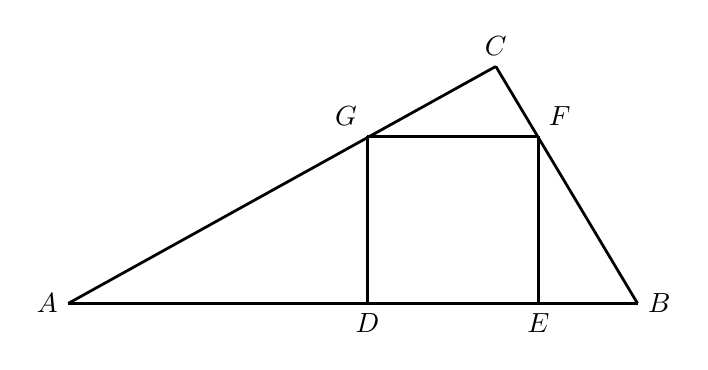
\begin{tikzpicture}[line join=round, line width=1.0pt]
  % Scale s = 0.012739 cm/px, origin at ink-bbox centre (362,198) px
  \coordinate (A) at (-3.61,-1.48);
  \coordinate (B) at (3.62,-1.48);
  \coordinate (C) at (1.82,1.53);
  \coordinate (D) at (0.19,-1.48);
  \coordinate (E) at (2.36,-1.48);
  \coordinate (G) at (0.19,0.64);
  \coordinate (F) at (2.36,0.64);

  % Base and sides
  \draw (A) -- (B);
  \draw (A) -- (C);
  \draw (C) -- (B);

  % Verticals and horizontal bar (GF spans exactly G to F; EF ends at F)
  \draw (D) -- (G);
  \draw (E) -- (F);
  \draw (G) -- (F);

  % Labels (font 10/12)
  \node[font=\fontsize{10}{12}\selectfont, left] at (A) {$A$};
  \node[font=\fontsize{10}{12}\selectfont, right] at (B) {$B$};
  \node[font=\fontsize{10}{12}\selectfont, above] at (C) {$C$};
  \node[font=\fontsize{10}{12}\selectfont, below] at (D) {$D$};
  \node[font=\fontsize{10}{12}\selectfont, below] at (E) {$E$};
  \node[font=\fontsize{10}{12}\selectfont, above left] at (G) {$G$};
  \node[font=\fontsize{10}{12}\selectfont, above right] at (F) {$F$};
\end{tikzpicture}
\end{document}